\chapter{Fundamento Te'orico}
\section{Dise'no del sistemas de control en espacio de estados}

\subsection{Asignaci'on de polos}

Todas las variables de estado con las que el sistema cuenta, se suponen medibles y disponibles para su realimentaci'on y si el sistema es completamente controlable, se pueden colocar los polos del sistema en cualquier posici'on dentro de una matriz de estado de ganancias (matriz de ganancias de a realimentaci'on de estados). Se consiguen estos polos a partir de la respuesta transitoria, as'i como de las respuestas de frecuencia. Seleccionando una matriz de ganancias apropiado se puede conseguir que los polos del sistema en lazo cerrado tengan una posici'on adecuada  \citep{ogata}.

\subsection{Dise'no mediante asignaci'on de polos}

Se deben especificar todos los polos en lazo cerrado del sistema, tomando en cuenta que para ello se deben tener medidas excelentes de las variables de estado o incluir un observador de estado en el sistema; a parte de que el requisito primordial es que el sistema sea completamente controlable \citep{ogata}.

Siendo un sistema de control con la forma:

\setlength{\parskip}{0.1cm}
\begin{center}
$
\left\lbrace
\begin{array}{ll}
\dot{x}=Ax+BU\\
y=Cx+DU
\end{array}
\right.
$
\end{center}
\setlength{\parskip}{0.1cm}
donde: $x=$vector de estado (vector de dimensi'on $n$)\\
			$y=$se'nal de salida (escalar)\\
			$u=$se'nal de control (escalar)\\
			$A=$matriz de coeficientes constantes $n*n$\\
			$B=$matriz de coeficientes constantes $n*1$\\
			$C=$matriz de coeficientes constantes $1*n$\\
			$D=$constantes (escalar)\\

Se selecciona la se'nal de control :
\begin{center} 
$u=-Kx$
\end{center}

Es decir que \textbf{u} es es un estado instant'aneo; siendo la matriz \textbf{K} de 1xn denominada como matriz de ganancia de realimentaci'on de estado. Sistema mostrado en la Fig. \ref{fig:siscerrado} \citep{ogata}.
\begin{figure}[ht]
	\centering
		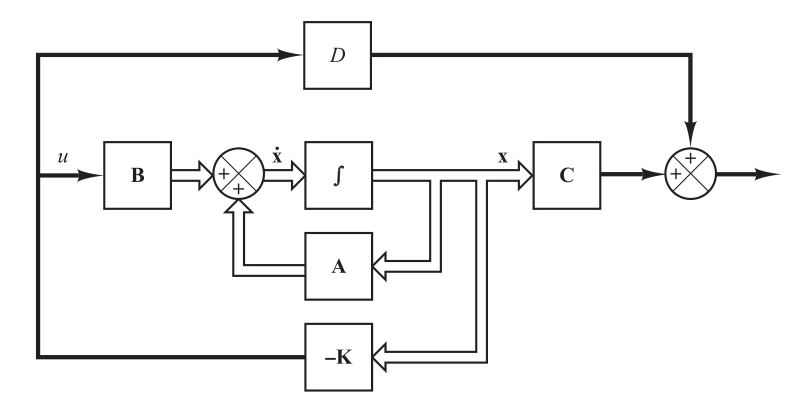
\includegraphics[scale=0.6]{sccerrado}
	\caption{Sistema de control en lazo cerrado}
	\label{fig:siscerrado}
\end{figure}

\setlength{\parskip}{0.4cm}

\section{Entorno de desarrollo integrado (IDE)}

El prop'osito m'as importante de un IDE es ayudar a acelerar el desarrollo preciso, r'apido y robusto de una aplicaci'on. Muchos IDEs se encuentran en desarrollo o est'an implementadas en universidades \citep{Ainternational}.

%%%%%%%%For most complex tasks, a combination of strategies is required. The ideal IDE will integrate shallow methods with methods based on tokens, patterns, grammars, keywords, logic, and finite state automata.It will integrate knowledge bases, expert systems, experts, planners, and other artificial intelligence systems with the overall framework 

\citet{kavitha} Muestra que algunos IDE contienen un compilador,int'erprete o ambos, como NetBeans y Eclipse. Muchos
IDEs modernos tambi'en tienen un navegador de clase,Y un diagrama de jerarqu'ia de clases.

\subsection{Entorno de desarrollo integrado abierto }

Open IDEs  son IDEs desarrollados, depurados y montados bajo una Licencia de Software de C'odigo Abierto, y permiten al programador de desarrollo de software nuevo, con todo tipo de licencias. Como PyCharm, NeatBeans, Matlab y otros.

\subsection{Herramientas de los IDEs }

``Hay muchas herramientas IDE disponibles para el c'odigo fuente
editor, herramientas de automatizaci'on y depurador. Algunos de los
Herramientas son, \textbf{\textsl{Eclipse,NetBeans, Code::Blocks, Code Lite, Dialog Blocks}}'' \citep{Ainternational}.
\begin{figure}[ht]
	\centering
		\includegraphics[scale=0.8]{idestop}
	\caption{Top 15 IDES. \smallskip Extraido de: \texttt{{http://pypl.github.io/IDE.html}}}
	\label{fig:idestop}
\end{figure}

Este top muestra la frecuencia con la que se realizan b'usquedas en IDE en Google. El 'indice puede ayudarle a decidir qu'e IDE utilizar \citep{pierre}. 

Como se puede ver en la Fig. \ref{fig:idestop} en la p'agina \pageref{fig:idestop}, est'an los IDE m'as importantes que se buscan en Google, y est'an  clasificadas por el lenguaje compatible como: ActionScript,	Ada,	Assembly,	BASIC,	C/C++,	C\#,	Common Lisp,	Component Pascal,	Eiffel,	Fortran, Haxe,	Java,	JavaScript,	Lua,	Pascal, Object Pascal,	Perl,	PHP,	Python,Racket,	Ruby,	Scala,	Small Basic,	Smalltalk,	Tcl.

En esta secci'on elegimos el lenguaje Python porque es una herramienta gratuita para el desarrollo y tambi'en es un lenguaje de programaci'on de alto nivel, de prop'osito general, interpretado y din'amico; todas estas particularidades hacen que este lenguaje sea perfecto para nuestro trabajo, y van a ser explicados en los siguientes cap'itulos.


\subsection{Software de c'odigo abierto}

El software de c'odigo abierto da acceso al c'odigo fuente; luego los usuarios pueden cambiar o modificar el producto original \citep{melissa}.

En otras palabras los usuarios tienen la libertad para ejecutar, copiar, distribuir, estudiar,
modificar y mejorar el software. Algunos autores lo
denominan ``software libre'' (tiene un contexto de libertad no de precio) \citep{anrango}. 

%%\subsubsection{Ideology}
%%%%%If you value fair use of information and intellectual freedom,
%open source software is right for you and your library. But
%remember, think of "free" as in freedom, not necessarily
%"free" as in price, although it often is. The free software
%movement differs slightly from open source software
%ideology in that free software promotes the freedom of all
%software everywhere and abhors proprietary software. Open
%source software proponents believe that this is not
%completely realistic and prefer promoting collaboration
%methods as superior to proprietary software. If a piece of
%software is called "free software," then it is also open source
%software. Live free, code free, improve the world \citep{melissa}.


\section{Lenguajes de programaci'on}
 
 
Lenguaje creado para para interpretar instrucciones elementales de la arquitectura mismo de los ordenadores; facilitando la tarea de programador, y que a partir de estos lenguajes se crean otros de nivel superior o lenguajes de alto nivel, que son mucho m'as productivos \citep{javier}.

 
\subsection{Paradigmas de programaci'on}

``Programming paradigms o Paradigmas de programaci'on'', seg'un \citet{javier} son patrones que moldean la forma de pensar y de formular soluciones asi como la de estructurar programas. Los paradigmas de programaci'on son: 
\begin{itemize}
\item Programaci'on imperativa. 
\item Programaci'on funcional. 
\item Programaci'on l'ogica. 
\item Programaci'on orientada a objetos.
\end{itemize}

\subsubsection{Lenguajes de alto nivel }
Del mismo modo \citep{javier} nos muestra que existen algunas caracter'isticas dentro de estos lenguajes:

Es un lenguaje independientes de la m'aquina, programas legibles y m'as f'aciles de entender; lenguajes m'as naturales; repertorio de instrucciones amplio, potente y f'acilmente utilizable;
 estructura pr'oxima a los lenguajes naturales, mantenimiento y correcci'on de errores m'as sencilla \citet{javier}.

\subsubsection{Traductores (Translators)}
Se establece que un traductor migra el programa creado de un lenguaje fuente a un lenguaje m'aquina. El proceso de conversi'on puede ser: por interpretaci'on o por compilaci'on \citep{javier}.
\subsubsection{Int'erpretes (Interpreters)}
Seg'un \citep{javier} es un programa que toma como entrada un programa escrito en lenguaje fuente y lo va
traduciendo y ejecutando instrucci'on por instrucci'on (de una en una).
\subsubsection{Compiladores (Compilers)}
Es un programa que toma como entrada un programa fuente y genera un programa
equivalente llamado programa objeto \citep{javier}.


\section{Python}
\subsection{Introducci'on}

Python nace en los noventa bajo la direccion de guido Van Rossum, es un lenguaje similar a Perl, pero con una sintaxis muy limpia y un c'odigo legible. Es un lenguaje interpretado, multiplataforma y orientada a objetos\citep{gonzales14}.

\subsection{Lenguaje interpretado o script}

Lenguaje que ejecuta un programa intermedio o de interpretaci'on en lugar de compilar a un lenguaje m'aquina, haciendo que este pueda ser interpretado directamente por la computadora. Python tiene muchas de las caracter'isticas de los lenguajes compilados, por lo que se podr'ia decir que es semi interpretado\citep{gonzales14}.


\subsection{Tipado din'amico}

Esta caracter'istica se refiere a que no es necesario declarar el tipo de dato de una variable, sino que este se determinar'a en tiempo de ejecuci'on; haciendo posible que el tipo de variable pueda cambiar con el tiempo \citep{gonzales14}.

\subsection{Tipado fuerte}

Es primordial convertir de forma expl'icita una variable a un nuevo tipo previo a su uso \citep{gonzales14}.

\subsection{Python}

Python deber'ia ser universal, su sintaxis es sencilla y clara; el tipado es fuerte, es orientada a objetos, tiene gran cantidad de librer'ias disponibles as'i como la calidad y potencia del lenguaje; por lo que desarrollar en python es una tarea sencilla \citep{gonzales14}.

Python es usado en Google, Yahoo, la NASA, Industrias Ligh \& Magic \citep{gonzales14}.

\begin{figure}[h]
	\centering
		
\includegraphics[scale=0.10]{Python_logo}
	\caption{Logo Python \texttrademark}
	\label{fig:Pythonlogo}
\end{figure}

\section{Sistemas operativos de tiempo real}

%\subsection{Introduction}

%Real­time and embedded computing applications in the first two computing era were rather rare and restricted
%to a few specialized applications such as space and defense. In the post­PC era of computing, the use of computer
%systems based on real­time and embedded technologies has already touched every facet of our life and is still growing
%at a pace that was never seen before. While embedded processing and Internet­enabled devices have now captured
%everyone's imagination, they are just a small fraction of applications that have been made possible by real­time
%systems. If we casually look around us, we can discover many of them ­ often they are camouflaged inside simple
%looking devices. If we observe carefully, we can notice several gadgets and applications which have today become indispensable to our every day life, are in fact based on embedded real­time systems. For example, we have ubiquitous
%consumer products such as digital cameras, cell phones, microwave ovens, camcorders, video game sets; telecommunication domain products and applications such as set­top boxes, cable modems, voice over IP (VoIP), and video
%conferencing applications; office products such as fax machines, laser printers, and security systems. Besides, we
%encounter real­time systems in hospitals in the form of medical instrumentation equipments and imaging systems.
%There are also a large number of equipments and gadgets based on real­time systems which though we normally do
%not use directly, but never the less are still important to our daily life. A few examples of such systems are Internet
%routers, base stations in cellular systems, industrial plant automation systems, and industrial robots \citep{mall}. 

%It can be easily inferred from the above discussion that in recent times real­time computers have become ubiquitous and have permeated large number of application areas. At present, the computers used in real­time applications
%vastly outnumber the computers that are being used in conventional applications. According to an estimate [3], 70\%
%of all processors manufactured world­wide are deployed in real­time embedded applications. While it is already true
%that an overwhelming majority of all processors being manufactured are getting deployed in real­time applications,
%what is more remarkable is the unmistakable trend of steady rise in the fraction of all processors manufactured
%world­wide finding their way to real­time applications \citep{mall}. 

%Some of the reasons attributable to the phenomenal growth in the use of real­time systems in the recent years 
%are the manifold reductions in the size and the cost of the computers, coupled with the magical improvements to
%their performance. The availability of computers at rapidly falling prices, reduced weight, rapidly shrinking sizes,
%and their increasing processing power have together contributed to the present scenario. Applications which not
%too far back were considered prohibitively expensive to automate, can now be affordably automated. For instance,
%when microprocessors costed several tens of thousands of Rupees, they were considered to be too expensive to be
%put inside a washing machine; but when they cost only a few hundred rupees, their use makes commercial sense \citep{mall}. 




\subsection{Definici'on}



As'i \citet{mall} define que un sistema se denomina sistema en tiempo real, cuando se necesita una expresi'on cuantitativa del tiempo (i.e. real-time) para describir el comportamiento de un sistema.

\citet{ortiz} nos brinda otro par de definiciones que son igualmente aceptables:

\begin{itemize}
	\item Un sistema a tiempo real debe producir tantas salidas como respuesta a unas entradas dentro de unos l'imites de tiempo plazos espec'ificos.
\item  Un sistema en tiempo real debe producir respuestas correctas dentro de unos limites de tiempo.
\end{itemize}

Pero de las cuales el mismo autor \citet{ortiz} se plantea un par de interrogantes derrivadas de estas definiciones, a las cuales 'el mismo da una respuesta:

\begin{itemize}
	\item ¿ Qu'e significa limites de tiempo espec'ificos?
	
	\begin{itemize}
		\item No necesitamos el mismo tiempo de respuesta en unas aplicaciones
que en otras.
	\end{itemize}
	\item¿ Por qu'e se dice ``debe producir'' y no dice ``produce''?

\begin{itemize}
	\item No en todas las aplicaciones es necesario que el sistema responda
siempre dentro de unos l'imites de tiempo concretos (ej. aplicaciones
multimedia), mientras que en otras es crucial (piloto autom'atico de
un avi'on).
\end{itemize}
\end{itemize}


\subsection{Aplicaciones}

Sobre las aplicaciones de los sistemas de tiempo real \citet{mall}  muestra algunos ejemplos, pero para el caso se presentaran solo dos ejemplos que ilustran la situaci'on de los sistemas operativos de tiempo real:

\subsubsection{Aplicaciones industriales}
Algunos ejemplos de aplicaciones industriales de sistemas en tiempo real son: sistemas de control de procesos, aplicaciones SCADA, equipos de prueba y medici'on, sistemas de automatizaci'on industrial y todos los materiales en equipos rob'oticos \citep{mall}.

\begin{itemize}
	\item \textbf{Ejemplo 1: Control de una planta qu'imica}\\
Un ordenador en tiempo real implementado en una planta qu'imica automatizada, monitorea peri'odicamente las condiciones de la planta como: lecturas actuales de presi'on, temperatura y concentraci'on qu'imica de la c'amara de reacci'on. Los par'ametros son muestreados peri'odicamente. Para mantener la reacci'on qu'imica a una determinada velocidad, la computadora en tiempo real decide las correcciones de las acciones necesarias, bas'andose en estos valores; cambiar la presi'on, temperatura u otros valores. En todos los sentidos, los l'imites de tiempo en un control de esta planta qu'imica var'ian desde unos pocos segundos hasta varios milisegundos \citep{mall}. 


\item \textbf{Ejemplo 2: Control, supervisi'on y Adquisici'on de Datos (SCADA )}\\
SCADA es una categor'ia de sistemas de control distribuidos que se utilizan en muchas industrias. Un sistema SCADA ayuda a supervisar y controlar un gran n'umero de eventos distribuidos de inter'es. En los sistemas SCADA, los sensores est'an dispersos en varios lugares geogr'aficos para recopilar datos en bruto (llamados eventos de inter'es). Estos datos se procesan a continuaci'on Y almacenados en una base de datos en tiempo real. Los eventos de inter'es est'an recibiendo datos de sensores en un sector espec'ifico dentro de una planta, luego se almacenan en una base de datos en tiempo real. Esta base de datos se est'a actualizando con frecuencia para convertirla en un modelo realista del estado de actualizaci'on del entorno. La restricci'on de tiempo en tal aplicaci'on SCADA es que los sensores deben detectar el estado del sistema a intervalos regulares (cada pocos milisegundos) y el mismo debe ser procesado antes de que se detecte el siguiente estado\citep{mall}.
\end{itemize}

Otros sistemas comunes de tiempo real dentro de algunas 'areas:

\begin{itemize}
	\item Sistemas de inyecci'on de conbustible multipunto.
	\item Impresora laser.

\item Video conferencias.
\item Celulares.
\item Sistemas de gu'ia de misiles.

\end{itemize}


\subsection{Modelo b'asico de un sistema en tiempo real}
\label{sec:ABasicModelOfARealTimeSystem}

\citet{mall}  explica el concepto b'asico sobre el modelo de un sistema en tiempo real:

\begin{figure}[ht]
	\centering
		\includegraphics[scale=0.7]{basic_realtimesystem}
	\caption{Modelo b'asico de un sistema en tiempo real}
	\label{fig:realtimesys}
\end{figure}

La Fig. \ref{fig:realtimesys} muestra un simple modelo b'asico de un sistema en tiempo real. \citet{mall} indica que  los sensores est'an interconectados con el bloque de acondicionamiento de entrada, que a su vez est'a conectado a la entrada interfaz. La interfaz de salida, el acondicionamiento de salida y el accionador est'an interconectados de una manera complementaria. A continuaci'on est'an brevemente los roles de los diferentes bloques funcionales de un sistema en tiempo real:

\textbf{Sensor:} Un sensor convierte alguna acci'on f'isica o caracter'istica de su entorno en se'nales el'ectricas \citep{mall}. 


\textbf{Actuador:} Un actuador es cualquier dispositivo que toma sus entradas de la interfaz de salida de un PC o microcontrolador y convierte estas se'nales el'ectricas en acciones f'isicas  \citep{mall}. 

\textbf{Acondicionamiento de se'nales:} \citet{mall} muestra que las se'nales el'ectricas producidas por un ordenador rara vez se pueden utilizar para accionar directamente un actuador por lo que es necesario algunos acondicionamientos realizados en se'nales brutas generadas por sensores y se'nales digitales generadas por computadoras.

\textbf{Conversi'on an'aloga-digital:} \citet{mall} explica que los ordenadores digitales no pueden procesar se'nales anal'ogicas. Por lo tanto, las se'nales anal'ogicas necesitan ser convertidas a forma digital. Las se'nales anal'ogicas pueden convertirse a forma digital utilizando un circuito cuyo diagrama de bloques se muestra en la Fig. \ref{fig:conversorad}. Utilizando el diagrama de bloques mostrado en Fig.\ref{fig:conversorad}, las se'nales anal'ogicas se convierten normalmente en forma digital a trav'es de los dos pasos principales siguientes:
\begin{figure}[ht]
	\centering
		\includegraphics[scale=0.8]{voltajecontinuo}
	\caption{Voltaje an'alogo continuo}
	\label{fig:voltajecontinuo}
\end{figure}


\begin{itemize}
	\item Muestra la se'nal anal'ogica (mostrado en la Fig. \ref{fig:voltajecontinuo}) a intervalos regulares. Este muestreo puede realizarse mediante un circuito de condensadores que almacena los niveles de voltaje. El nivel de voltaje almacenado puede ser discretizado. Despu'es de muestrear la se'nal anal'ogica, una forma de onda escalonada como se muestra en la Fig. \ref{fig:voltajedis} es obtenida \citep{mall}. 
\item Convierte el valor almacenado en un n'umero binario utilizando un convertidor anal'ogico a digital (ADC) como se muestra en la Fig. \ref{fig:conversorad} y almacenar el valor digital en un registro \citep{mall}. 

\end{itemize}

\begin{figure}[ht]
	\centering
		\includegraphics[scale=0.5]{voltajediscreto}
	\caption{Voltaje an'alogo convertido a la forma discreta}
	\label{fig:voltajedis}
\end{figure}

\begin{figure}[ht]
	\centering
		\includegraphics[scale=1]{conversorad}
	\caption{Conversi'on de una se'nal an'aloga a n'umero digital de 16 bits.}
	\label{fig:conversorad}
\end{figure}



\subsection{Tipos de tareas en tiempo real}

\subsubsection{Tareas del tipo hard}
Una tarea del tipo hard en tiempo real es aquella que est'a limitada a producir sus resultados dentro de ciertos l'imites de tiempo predefinidos. Se considera que el sistema ha fallado cuando alguna de sus tareas en tiempo real no 
produce los resultados requeridos antes del l'imite de tiempo especificado \citep{mall}. 
	
\subsubsection{Tareas del tipo firm }
Cada tarea en tiempo real del tipo firm est'a asociada con alg'un plazo predefinido antes del cual se producen sus resultados. Sin embargo, a diferencia de una tarea en tiempo real hard, incluso cuando una tarea en tiempo real firm no completa dentro su plazo la tarea requerida, el sistema no falla. Los resultados tard'ios son simplemente descartados. En otras palabras, la utilidad de los resultados calculados por una tarea en tiempo real firm se convierten en cero despu'es de la fecha l'imite. Se puede decir que si la respuesta en tiempo de una tarea excede el plazo especificado, entonces la utilidad de los resultados se convierte en cero y los resultados se descartan \citep{mall}.
\section{Open Hardware}

\subsection{Definici'on}

Aplicando ciertas libertades y definiciones antes dadas al software libre, entre ellas: libertad de uso, modificaci'on, distribuci'on y la redistribucion en mejoras con base al software original, con la diferencia de que para obtener un producto tangible tuvo que haber de antemano un sistema o proyecto con planos, estudios de costo, entre otras cosas. \citep{hernando}.

\citet{russell} presenta un resumen m'as espec'ifico sobre el "hardware abierto": El hardware de c'odigo abierto es un tipo de hardware en el que los esquemas y dise'nos se hacen sin restricciones y est'an disponibles para todos.
\subsection{Propiedades}
\citet{russell} da algunas propiedades del hardware abierto: Primero se acompa'nan a menudo del software abierto; Esto puede aportar fiabilidad y facilidad de depuraci'on. En segundo lugar Open Hardware viene con desarrollo modular para prototipos r'apidos usando bibliotecas preescritas.

El hardware de c'odigo abierto es hardware cuyo dise'no se hace disponible p'ublicamente para que cualquier persona pueda estudiar, modificar, distribuir, fabricar y vender el dise'no o el hardware basado en ese dise'no \citep{russell}.

\subsubsection{Hardware de c'odigo abierto}
Se refiere al hardware para el cual toda la informaci'on del dise'no se pone a
disposici'on del p'ublico en general. Open source hardware se puede basar en un
free hardware design, o el dise'no en el cual se basa puede ser restringido de
alguna manera  \citep{hernando}.

\subsubsection{Hardware libre}
Es un t'ermino usado de vez en cuando como sin'onimo para el open source
hardware; la cual busca ser directamente paralelo entre el hardware y el software. El t'ermino de
free hardware es particularmente confuso puesto que implica el estado f'isico del
hardware, m'as que su dise'no, el cual  es libre de alguna manera. Esto no es del
todo cierto en el sentido del costo, y tiene poca importancia en el sentido social.
Lo m'as simple es evitar este t'ermino totalmente, exceptuando su significado de
costo   \citep{hernando}.

\subsection{Hardware libre en Ecuador}
El inter'es de los modelos de Hardware Libre para Ecuador procede de su potencial como r'egimen de
producci'on y distribuci'on de tecnolog'ia, as'i como del desarrollo de nuevos
v'inculos sociales en torno a ella. El Hardware Libre tiene notables ventajas
comparativas, la situaci'on de partida del pa'is invita a prestar atenci'on al desarrollo de hardware libre con el objetivo de que su expansi'on favorezca el crecimiento econ'omico del en Ecuador, sin que tal desarrollo limite el
brillante potencial del Hardware Libre para la econom'ia del pa'is  \citep{lazalde}.


Actualmente existen muchos problemas para el desarrollo de un
hardware sustentable. Uno de los principales problemas son los altos costos de producci'on,
habitualmente derivados de la dependencia tecnol'ogica que afecta a muchos pa'ises, como
Ecuador \citep{lazalde}.

Por otra parte, los fabricantes de hardware y los titulares de los derechos de
autor aplican la Gesti'on de Derechos Digitales (DRM, por sus siglas en
ingl'es) para controlar el uso de contenidos y dispositivos digitales \citep{lazalde}.

Frente a esto, el Hardware Libre es relativamente barato y est'a profundamente integrado en los niveles de
alta innovaci'on. Adem'as, puede ser f'acilmente modificado a fin de
servir ciertos prop'ositos educativos \citep{lazalde}.


\section{Arduino}
\subsection{Introducci'on}
Entre las implementaciones de HL (Hardware Libre) m'as representativas est'a Arduino, una plataforma
inform'atica basada en un tablero microcontrolador simple y un ambiente de desarrollo para
escribir software en 'el. Est'a dirigido a artistas, dise'nadores, aficionados y
dem'as interesados en crear dispositivos o ambientes interactivos. Este microcontrolador
permite el funcionamiento de varios dispositivos derivados como el Arduino Geiger
(detector de radiaci'on), pHduino (medidor de pH), Xoscillo (osciloscopio) y OpenPCR
(an'alisis de ADN) \citep{lazalde}.

\citet{lazalde} exponen que Arduino bajo la licencia de Creative Commons "Attribution ShareAlike 3.0" (2010), lo que
significa que:
\begin{itemize}
	\item Quienquiera puede producir copias, redise'narlo o incluso vender placas de hardware.

\item Quienquiera que vuelva a publicar el dise'no de referencia debe atribuirlo al equipo original de Arduino.

\end{itemize}

\subsection{Asp'ectos T'ecnicos}


\citet{garcia} especifica la conformaci'on del Arduino :
El Arduino UNO es muy popular por su sencillez, coste y
dimensiones. Utiliza el microcontrolador ATmega328P, fabricado por ATMEL. Cuanta con las siguientes caracter'isticas t'ecnicas:

\begin{itemize}
	\item Voltaje: 5V.
\item Voltaje de entrada (recomendado): 7-12V.
\item Voltaje de entrada (l'imites): 6-20V.
\item Pines de entradas y salidas digitales: 14.
\item Corriente en pines de entrada y salida: 40mA.
\item Pines de entrada anal'ogica: 6.
\item Corriente en pin de 3.3V: 50mA.
\item Memoria Flash: 32KB.
\item SRAM: 2KB.
\item EEPROM: 1KB.
\item Velocidad reloj: 16MHz.
\item Dimensiones: 68.6x53.4mm.
\end{itemize}

\subsubsection{Arduino UNO Pinout Diagram}
\begin{figure}[h]
	\centering
		\includegraphics[scale=0.60]{Descripcionpines1}
	\caption{Arduino UNO Pinout Diagram}
	\label{fig:Descripcionpines}
\end{figure}
EL arduino IDE al momento de esta investigaci'on se encuentra en la versi'on 1.6.12 en su p'agina oficial.

\subsection{Arduino en Ecuador}
En Ecuador los estudiantes son los principales impulsodores del
desarrollo de proyectos de hardware libre. En la Campus Party celebrada en Quito en 2013, estudiantes
de la Universidad Polit'ecnica de Chimborazo, la Universidad T'ecnica de Loja y la
Universidad Salesiana de Quito desarrollaron dispositivos electr'onicos basados en Arduino.
Un ejemplo de Hardware Libre producido en el Ecuador es la aeronave no tripulada llamada Gavil'an UAV-2, dise'nada por las Fuerzas A'ereas Ecuatorianas (FAE) para vigilancia de 'areas de dif'icil acceso como la selva \citep{lazalde}.


\section{Red de 'area de comunicaci'on (CAN)}

\subsection{Can Bus Shield para Arduino: aspectos t'ecnicos}

El hardware que va a ser embebido en la placa de Arduino es un shield de marca SPARK FUN (CAN COMMUNICATION):
\begin{figure}[ht]
	\centering
		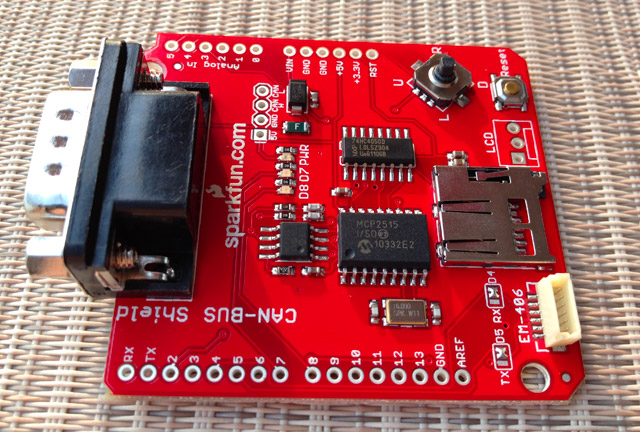
\includegraphics[scale=0.4]{shieldcan}
	\caption{CAN bus shield Sparkfun}
	\label{fig:sparkfun}
\end{figure}

Permite montar la red CAN con 4 nodos incrustados en ella. Consta de las siguientes caractr'isticas:

\begin{itemize}
	\item CAN v2.0B up to 1 Mb/s (1000Kbps).
	\item High speed SPI Interface (10 MHz) (with Arduino´s shield).
	\item Standard and extended data and remote frames.
	\item CAN connection via standard 9-way sub-D connector (DB-9).
	\item Power can supply to Arduino by sub-D via resettable fuse and reverse polarity protection.
	\item Socket for EM506 GPS module.
	\item Micro SD card holder.
	\item Connector for serial LCD.
	\item Reset button.
	\item Joystick control menu navigation control.
	\item Two LED indicator.
\end{itemize}
\begin{figure}[ht]
	\centering
		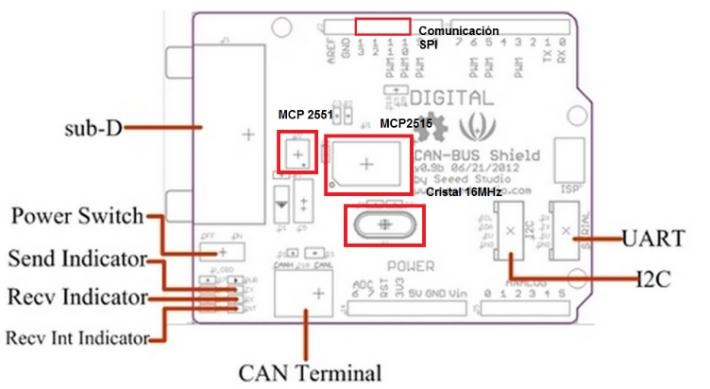
\includegraphics[scale=0.6]{canpartes}
	\caption{Partes del Shield CAN}
	\label{fig:canpartes}
\end{figure}





\subsection{Introducci'on}

El bus CAN  surge de la necesidad encontrar una forma de interconectar y conectar los distintos dispositivos de un autom'ovil en una sola red de una manera sencilla y reduciendo significativamente las conexiones, luego estandarizada en la norma ISO 11898-1; CAN bus cubre la capa de Enlace de datos y la F'isica  dentro de la pila de protocolo OSI \citep{garcia}.

%\begin{figure}[h]
	%\centering
		%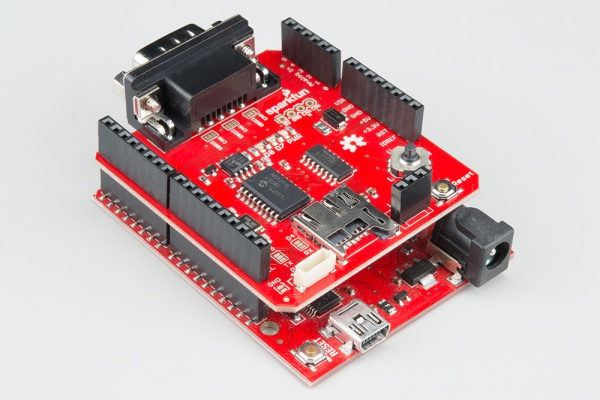
\includegraphics[scale=0.45]{canarduino}
	%\caption{\textit{CAN-BUS Shield} montado en un Arduino}
	%\label{fig:canarduino}
%\end{figure}


\subsection{Capa de enlace}
El protocolo de acceso es CSMA/CD + AMP (Carrier Sense Multiple
Access/ Collision Detection + Arbitration on Message Priority). Bajo este protocolo, los medios se ponen a la escucha de tramas de datos enviados en la red desde cualquier nodo, evitando as'i enviar mensajes mientras la red est'a ocupada; en el caso de que se envien mensajes al mismo tiempo desde dos o mas puntos de la red, el mensaje enviado es el que tenga como emisario al del identificador m'as bajo; cada nodo tiene un identificador que deber'a ser 'unico, es designado por software \citep{garcia}.


El campo de desici'on es al principio de la trama y la desici'on de prioridad se toma al final de la misma como se ve a continuaci'on:

\begin{figure}[ht]
	\centering
		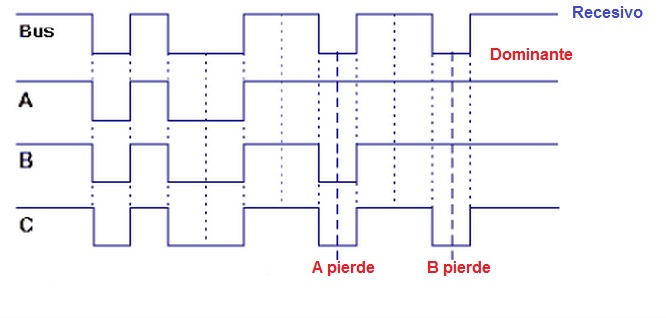
\includegraphics[scale=0.6]{Canynodos}
	\caption{Buffer de salida. Obtenido de \citet{garcia}.}
	\label{fig:canynodos}
\end{figure}

\subsection{Capa f'isica}

La capa f'isica debe recibir y enviar mensajes a la vez; a dem'as de presentar el estado recesivo y dominante en los nodos. tiene tres sub capas:

\subsubsection{PSL}
Physical Signaling Layer, sincroniza y temporiza los bits (modificaci'on por software) \citep{garcia}.
\subsubsection{PMA}
Convierte los niveles l'ogicos de transmisi'on y recepci'on  al lenguaje del protocolo \citep{garcia}.

\begin{figure}[ht]
	\centering
		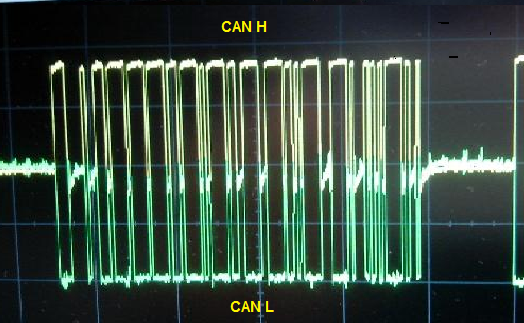
\includegraphics[scale=0.6]{canhcanl}
	\caption{Forma de onda generada por los canales de salida CAN H y CAN L \citep{garcia}.}
	\label{fig:canhcanl}
\end{figure}

La diferencia entre CAN H y CAN L que provee la comunicaci'on va de 0 a 2 volts, lo que da un nivel logico a un bit; el modo diferencial permite eliminar ruido \citep{garcia}.

\subsubsection{MDI}

Medium Dependent Interface, o interfaz dependiente del medio, indica como y bajo que medio se har'a la transmisi'on \citep{garcia}.

\begin{itemize}
\item Cables con resistencias de 120 $ \Omega $ .
\item Cable trenzado o apantallado.
\item Evitar derrivaciones.
\end{itemize}

\subsubsection{Trama de CAN bus}

El siguiente gra'afico representa una trama de datos de la comunicaci'on CAN:

\begin{figure}[ht]
	\centering
		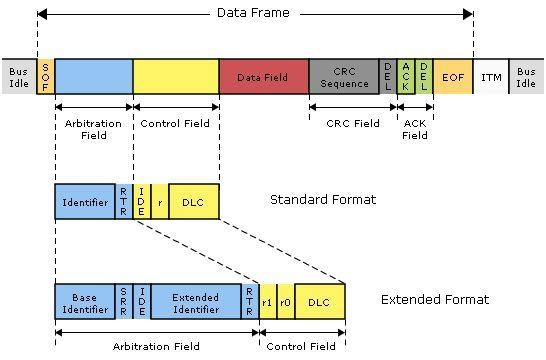
\includegraphics[scale=0.8]{tramacan}
	\caption{Trama generada en la comunicaci'on CAN\citep{garcia}.}
	\label{fig:tramacan}
\end{figure}

Consta de los siguientes elementos:

\begin{itemize}
\item SOF (Start of Frame bit).
\item Campo de arbitrio.
\item Campo de control.
\item Campo de datos.
\item Campo de verificaci'on por redundancia c'iclica CRC.
\item Campo de reconocimiento.
\item Campo de fin de trama.
\end{itemize}


\subsubsection{Trama remota}
Un nodo tiene la capacidad de solicitar un mensaje de otro nodo usando tramas remotas. Luego el nodo enviara su informaci'on al solicitante; el nodo que solicite la informaci'on deber'a tener el mismo identificador \citep{garcia}. Este tipo de trama no ser'a usada en el presente trabajo; en su lugar se utilizar'a una trama estandar de 8 bytes de datos.



\section{Driver, encoder, motor y finales de carrera}

El driver a utilizarse es DRIVER VNH2SP30, driver de hasta 16 volts. El encoder es HEDM-5500 con una resoluci'on de 2000 puntos cada 360° (2 encoders). El motor dc tiene una potencia de 180 watts a 24 volts. Finales de carrera del tipo mec'anico. Todos estos sensores y actuadores est'an descritos por \citet{montalvo} en la tesis previa a este trabajo y est'an montadas en el sistema mec'anico.